\chapterimage{Figures1_3/aux_optics1_3.png} % Chapter heading image
%PMC bench in the 10m AEI prototype copyright AEI
\chapter{Auxiliary Optics}
%\section{Auxiliary Optics}
\label{sec:Aux-optics}

\begin{samepage} % Latex vodoo to not waste half the first page

We use the term \emph{auxiliary optics} here for any optical subsystem not otherwise covered by a specific category (e.g. core optics or light sources). We further sub-categorize into these subsystems:
The {\bf Input Optics} subsystem includes all optics between the main light source and the input of the core interferometer, typically defined by the power recycling mirror. The {\bf Output Optics} subsystem includes all optics between the core interferometer output (typically defined by the signal recycling mirror) and the photo-detectors which detect the gravitational wave signal, with the exception of specific optical components used for the generation of squeezed light. The {\bf Active Wavefront Control} subsystem includes means for sensing and actively controlling the spatial properties of interferometer beams, with the typical goal of minimizing mode matching losses and contrast defects. The {\bf Stray Light Control} subsystem encompasses all design features which are intended to reduce the impact of stray light on detector operations. Finally, the subcategory {\bf Other Auxiliary Optics} catches optics that fall neither into the other larger categories or the above 
% auxiliary optics 
subcategories.

\section{State of the Art}
The {\bf Input optics} subsystem is responsible for delivering the laser light from the pre-stabilized laser (PSL) system to the core interferometer in the correct spatial mode, with the necessary phase modulation sidebands, and with the required frequency, intensity and alignment stability. This subsystem therefore typically includes an electro-optic modulator (EOM) for producing the phase modulation, one or more suspended input mode cleaner (IMC) cavities, a power control system, and an input Faraday isolator (IFI) to protect the PSL from light reflected from the main interferometer. Detailed descriptions of the IO subsystems of \ac{aLIGO}  and AdVirgo can be found in Refs.~\cite{aLIGO_IO,IOchapter}. 

\end{samepage} % Latex vodoo to not waste half the first page

% In \ac{2G}  detectors, 
The {\bf Output optics} subsystem is responsible for filtering out higher-order spatial modes and unwanted control sidebands from the interferometer output light, and delivering the beam to the photodetectors where the gravitational-wave signal measurement is made. The recent and planned squeezed light upgrades expand the role of this subsystem to include delivery of the squeezed beam to the main interferometer. This subsystem typically includes an output Faraday isolator, an output mode cleaner cavity (OMC), and high quantum efficiency photodiodes.

\noindent {\bf \ac{AWC}} is used in gravitational-wave detectors to compensate for thermal effects caused by the absorption of light in the interferometer core optics. As the circulating light power goals increased from 1st to 2nd generation detectors, so too did the requirements for compensation of these thermal effects. The \ac{2G}  detectors have all implemented a range of active wavefront control methods including ring heaters, CO$_2$ laser heating, thermal radiation projection, and thermally deformable mirrors~\cite{aLIGO_AWC, AdVirgo_IO}. This subsystem is often conflated with the \ac{TCS}, although \ac{TCS} constitutes only a part of the \ac{AWC} system. 

\noindent {\bf Stray Light Control}
mitigates the effects on the sensitivity of the detector of light that is scattered out of the main beam and then scattered by another surface back into it. 
% as that can cause noise that can limit the sensitivity of the detector.
Many precautions are taken in gravitational-wave detectors to minimize the amount of light scattered out of the beam (by using high-quality smooth optical surfaces everywhere), and also to minimize the available paths for re-entry of scattered light into the main beam (by using baffles wherever possible). 

\noindent 
Examples of {\bf "Other Auxiliary Optics"} include the auxiliary length sensing (ALS) systems for pre-stabilizing the arm cavities, and optical levers for local sensing of the alignment of optics.

\section{Requirements, Challenges and Current/Planned R\&D }
\noindent{\bf{Input optics}}
 % Future \ac{3G}   GW detectors will require different input optics than the current second-generation detectors. 
Terbium gallium garnet The ways in which the \ac{3G}   detector input optics will differ from the current ones depends heavily on some of the design decisions for \ac{3G}   detectors, many of which have not yet been made. Most critical for the input optics will be the choice of laser wavelength; the \ac{EOM} and \ac{IFI} rely on unusual electro- and magneto-optic materials that may have significantly different characteristics at longer wavelengths. Choosing suitable materials is not expected to pose a great challenge if the wavelength is changed to 1550\,nm, but 2+$\mu$m will probably require considerable effort. The high power transmitted through these optics makes low absorption critical (due to the resulting thermal lensing and depolarization effects), thus further narrowing the choice of suitable material. At 2$\mu$m Faraday isolators already exist~\cite{EOTFI}, but a high power vacuum compatible one must be developed as it is not commercially available. Iron garnets should be considered as potential candidates for the magneto-optic material for 2+$\mu$m light, also having the advantage that the Faraday rotation effect is an order of magnitude larger than that of \ac{TGG}  in the near infrared range, allowing a reduction in magnet size and the overall footprint and weight of the device.
The \ac{IMC} design is not expected to fundamentally change beyond the 2nd generation.  However, AdVirgo and \ac{aLIGO}  both have significant noise contributions from beam jitter~\cite{aLIGOjitter,adVirgojitter}. Increasing the \ac{IMC} finesse or adding a second \ac{IMC} in series with the first could be a way to further suppress the beam jitter. Another possibility is to reduce the beam jitter at the source, either passively or with 
% high bandwidth 
control loops.  

In addition to upgrades and modifications of existing IO components, several new components are also being researched. High bandwidth electro-optic beam deflectors could be used as actuators for beam jitter suppression loops and for providing alignment sidebands for an alternative method of alignment sensing in both the \ac{IMC} and in the core interferometer~\cite{RFJASC}. The use of higher-order modes for coating thermal noise reduction is still under consideration for \ac{3G}   interferometers~\cite{LGmodes}. If this technology is pursued further, the higher-order mode preparation path is likely to be incorporated into the IO remit. The use of complex modulation~\cite{complexmod} and parallel modulation~\cite{kagraMZI} are also under investigation for reducing sidebands-of-sidebands effects that may limit interferometer sensing and control performance.

\noindent{\bf{Output optics}}
With all \ac{3G}   concepts assuming significant enhancement from the use of squeezed light, the critical feature for the \ac{3G}   output optics will be ultra-low optical losses~\cite{squeeze_lossbudget}. \acp{OFI} with reduced optical losses are being developed~\cite{EGOLLFI,UFLLFI}.
% , for use in the advanced GW detectors. 
\Acp{OMC} must also be designed for high throughput, and photodetectors must have high quantum efficiency (QE). High-QE photodetectors at longer wavelengths have been identified as a crucial \ac{RaD}  task; one which may be especially onerous for 2+$\mu$m light. 
Frequency dependent squeezing will also require the inclusion of a \ac{FC} in the path between the squeezed light source and the OFI. 300\,m long \acp{FC} are planned for the near-term upgrades to \ac{aLIGO} and \ac{AdVirgo}, following on from \ac{RaD} ~\cite{MITFC,TAMA_FDS2016}.
%performed at MIT~\cite{MITFC} and in Japan~\cite{TAMA_FDS2016}. 
Alternative readout schemes such as \ac{BHD} (another project planned for inclusion in \ac{A+}) will require a redesign of the output optics chain~\cite{BHD}. There is also a need to develop robust length and angular control schemes for detuned filter cavities.
% and finesse control to control pole frequency.

%\begin{figure}[htb]
%\centering
%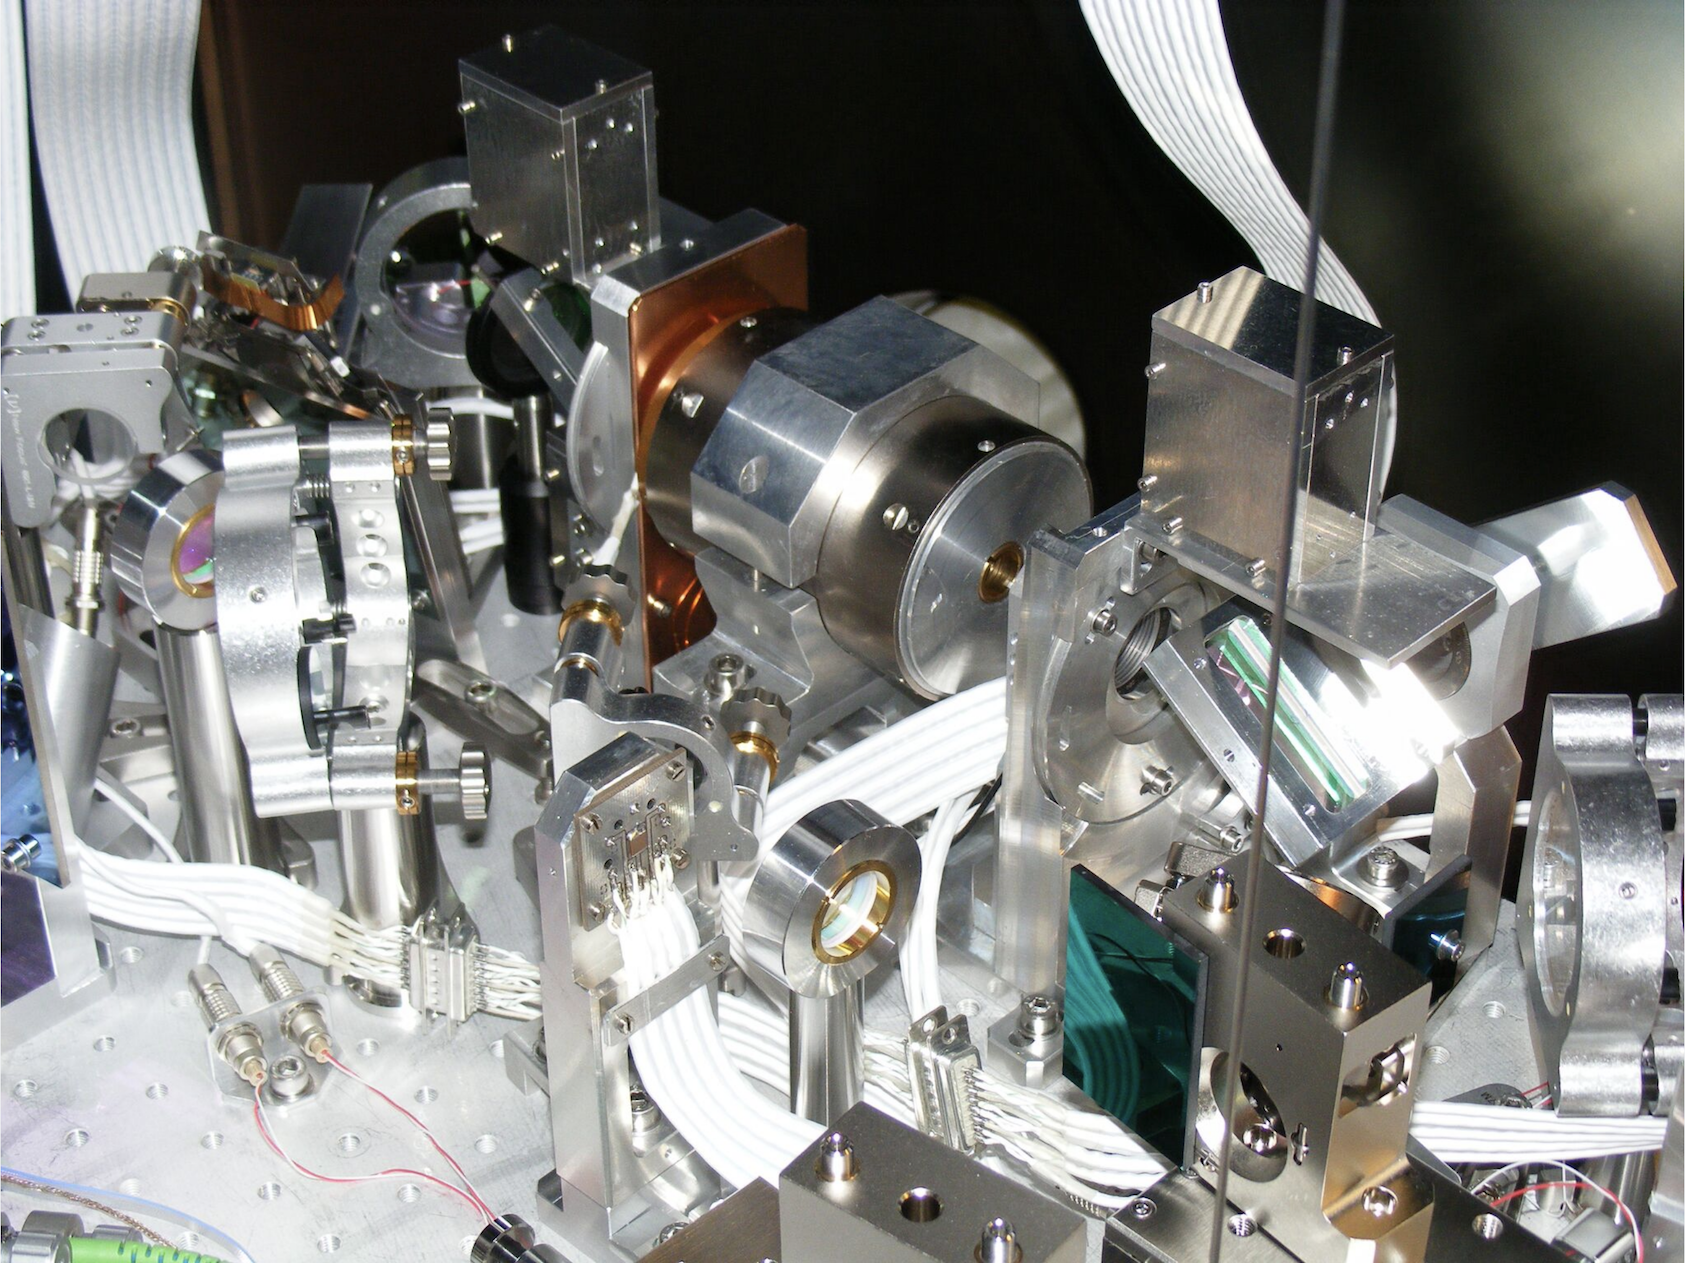
\includegraphics[width=0.6\textwidth]{Figures/LLFI.png}
%\caption{The low-loss OFI upgrade to Advanced Virgo, recently installed ahead of the third observing run of the advanced detector era.\label{fig:AdVLLFI}}
%\end{figure}\magentacomment{Do we want to have this figure here. I does not add much information and is the only figure in all chapters; except intro. On the other hand it would not shorten the chapter, as it does not gain a full page}
\noindent{\bf{Active wavefront control}}
In \ac{1G} and \ac{2G} detectors, \ac{AWC} has often been implemented in something of an \emph{ad hoc} way. In no cases has a feedback loop been used to maintain mode matching in a detector during normal operations. This is partly due to the low bandwidth of the typical actuators, but also due to the limitations in the \ac{AWC}  sensors available. As a result, \ac{AWC}  is typically employed in a set-and-forget manner, which requires frequent manual retuning as the circulating power in the interferometer changes. \ac{3G}   detectors will likely require higher performance from the \ac{AWC}  subsystem for several reasons: higher circulating powers, larger thermal gradients under cryogenic operation, larger beams with flatter wavefronts, and stricter requirements on optical losses. An \ac{LSC} white paper on \ac{AWC}  has been written to track the LSC \ac{RaD}  in this direction~\cite{aLIGO_AWC}, and similar work is planned for AdVirgo+. \ac{AWC}  \ac{RaD}  for \ac{3G}   detectors is expected to focus on new sensors (\ac{RF} bullseye wavefront sensors~\cite{bullseye}, improved Hartmann wavefront sensors~\cite{HWS}, phase cameras~\cite{phasecam}), as well as actuators (converting existing actuators for new optic materials, and developing new actuators). 

\noindent{\bf{Stray light control}}
Although it is often difficult to diagnose directly, stray light was likely limiting the sensitivity of both \ac{aLIGO}  and AdVirgo during O2. As such, improvements must clearly be made in order to reach \ac{3G}   sensitivities. 
% with any methods other than extending the baseline length. 
Continued \ac{RaD}  into mirror polishing and coating techniques to give improved surface roughness will go some way to reducing stray light contributions, as will the development of better baffling materials with lower reflectivities. One concern is that if the laser wavelength is changed to 2+$\mu$m, it may be difficult to find good absorbers for baffle materials. The quieter \ac{3G}   infrastructure environments may allow relaxing some scattering performance requirements.

\noindent{\bf{Other auxiliary optics}}
AdVirgo, \ac{aLIGO}  and \ac{KAGRA}  all either use (or provision for) an auxiliary length sensing system in order to make the interferometer locking process deterministic. Since the optical layout of \ac{3G}   detectors is not expected to reduce in complexity, it seems natural that similar systems will be required in the future. Optical levers are omnipresent in \ac{2G}  detectors, and provide important information about angular motion of the optics. Increased sensitivity in these local sensors may be beneficial for \ac{3G}   detectors
% with increased baselines and sensitivity goals, 
and \ac{RaD}  is ongoing towards that end. \Ac{SPI}~\cite{SPI}, which is currently being used at the \ac{AEI} 10\,m prototype, may be a useful technique for reducing low frequency control noise in \ac{3G}   detectors, and will require an additional auxiliary optical subsystem.

\section{Pathways, Required Facilities, Collaborations and Mechanisms}

Much of the auxiliary optics subsystems \ac{RaD} , such as materials investigations for \acp{EOM} and \acp{FI}, can be performed in small laboratories. 
Some of the larger subsystems such as filter cavities, on the other hand, require larger integrated facilities for testing. In many cases, the development of \ac{3G}   auxiliary optics technologies is also beneficially incorporated into the modernisation of second-generation detectors. By virtue of being \emph{auxiliary}, modular, incremental upgrades in many of these technologies are possible. Modular upgrades are not feasible in the case of a change in the main laser wavelength, however. Such a change for \ac{3G}   detectors will necessitate a broader range of auxiliary optics \ac{RaD} , which would benefit from a more complete demonstration on prototype detectors or finally at full scale in Voyager.

\section{Outlook and Recommendations}
%Activities on Input Optics and Output optics are relatively  well covered and organized within the existing collaborations. 
%Active wavefront control and stray light control would benefit greatly from increased global collaboration. 
%Due to the ad hoc nature of the development of these subsystems to date many groups have taken individual paths to different but often similar solutions. We propose the formation of global working groups in these areas. 

Activities on Input Optics and Output optics are relatively well covered and organized within the existing collaborations. Active wavefront control and stray light control would benefit greatly from increased global collaboration. Due to the ad hoc nature of the development of these subsystems to date many groups have taken individual paths to different but often similar solutions. Many of the auxiliary optics subsystems will be strongly impacted by the choice of laser wavelength. Beyond this, the input optics has a direct interface with the light source, and so information exchange between groups performing \ac{RaD}  in these two areas will be critical. The output optics subsystem will be closely linked to the quantum noise working groups as squeezing is foreseen in all future detectors. 

We recommend:
\begin{itemize}
\item the formation of global working groups across the different auxiliary subsystems to coordinate and focus development
\item  that mechanisms be put in place to facilitate close collaboration between groups working on auxiliary optics, light sources and quantum noise.  This would be facilitated by the formation of a global \ac{3G}   \ac{RaD}  planning committee.
\end{itemize}
While auxiliary optics are largely modular, enough time must be given between the selection of a laser wavelength and construction for the required \ac{RaD}  to conclude for auxiliary optics. Given the current \ac{RaD}  progress, this lead time could be five years. 


%\greencomment{Stan: clarify the recommendations}

%The below is informed by a survey of research groups who are working on, or have previously worked on auxiliary optics topics~\cite{AuxActivitiesTable}.

%\noindent{\bf Input optics} The groups working on IO for 2nd generation upgrades and beyond are primarily those groups who have worked on providing input optics for aLIGO, AdVirgo, GEO\,600 and \ac{KAGRA}  in the past. In the LSC-Virgo collaboration information is shared on progress in development of future input optics mostly through the auxiliary optics working group, with talks and posters at collaboration meetings. This method of collaboration seems to be sufficient for now. If the community steers towards a change in wavelength, however, additional information exchange mechanisms may be required in order to accelerate the development of suitable input optics components.

%\noindent{\bf Output optics} The main feature of upgrades of the second generation output optics and beyond is the minimization of optical losses while adding further subsystems such as filter cavities and balanced homodyne detection paths. 
%Low-loss Faraday isolators are advantageous for short-term \ac{2G}  detector upgrades, so it certainly would be useful for the 5 identified groups to work together and hold dedicated workshops to discuss progress and plans in the near future. 

%\noindent{\bf Active wavefront control} 
%This subsystem was identified by the authors as one that could benefit from increased global cooperation. Due to the \emph{ad hoc} nature of the development of this subsystem to date, many groups have taken individual paths to different but often similar solutions. We propose forming an active wavefront control subgroup to focus efforts on a common goal of appropriate wavefront sensors and control strategy for future detectors. 

%\noindent{\bf Stray light control} This subsystem could benefit from collaboration between groups worldwide, as the needs for establishing requirements for reflectivity and residual motion of baffles, raytracing for the \ac{3G}   instruments, and lessons learned from the \ac{2G}  instruments all are mostly common.


%especially if the laser wavelength chosen is the same for all of the next generation detectors. If each project uses different wavelengths, \ac{RaD}  overlap will be much smaller. 
% If different choices are made, each project should organize \ac{RaD}  activities on their own. 
%Thus, from the stray light control perspective at least, significant savings in time and money could be made by choosing common wavelengths among \ac{3G}   detectors. 

%\noindent{\bf Other auxiliary optics} Unless required by groups working on auxiliary optics topics outside the scope of the above, specific collaboration mechanisms are not seen as a priority at this time. 

%\noindent{\bf Collaborations between AO and other subsystems}
% \noindent{\bf Light sources} 
Many of the auxiliary optics subsystems will be strongly impacted by the choice of laser wavelength. Beyond this, the input optics has a direct interface with the light source, and so information exchange between groups performing \ac{RaD}  in these two areas will be critical.
% \noindent{\bf Quantum noise} 
The output optics subsystem will be closely linked to the quantum noise working groups as squeezing is foreseen in all future detectors. Close collaboration between these groups will therefore be beneficial.

%\section{Roadmap and timeline}
While auxiliary optics are largely modular, enough time must be given between the selection of a laser wavelength and construction for the required \ac{RaD}  to conclude for auxiliary optics. Given the current \ac{RaD}  progress, this lead time could be five years. 
